% ──────────────────────────────────────
%  NeSy-Mamba Architecture Diagram
%  Standalone TikZ (compile separately or \input{} into main.tex)
% ──────────────────────────────────────
\documentclass[border=5pt]{standalone}
\usepackage{tikz}
\usetikzlibrary{positioning, arrows.meta, fit, calc, decorations.pathreplacing}
\usepackage{amsmath,amssymb}

\definecolor{mamba}{RGB}{52,101,164}
\definecolor{slot}{RGB}{204,102,0}
\definecolor{loss}{RGB}{164,0,0}
\definecolor{embed}{RGB}{78,154,6}
\definecolor{head}{RGB}{117,80,123}

\begin{document}
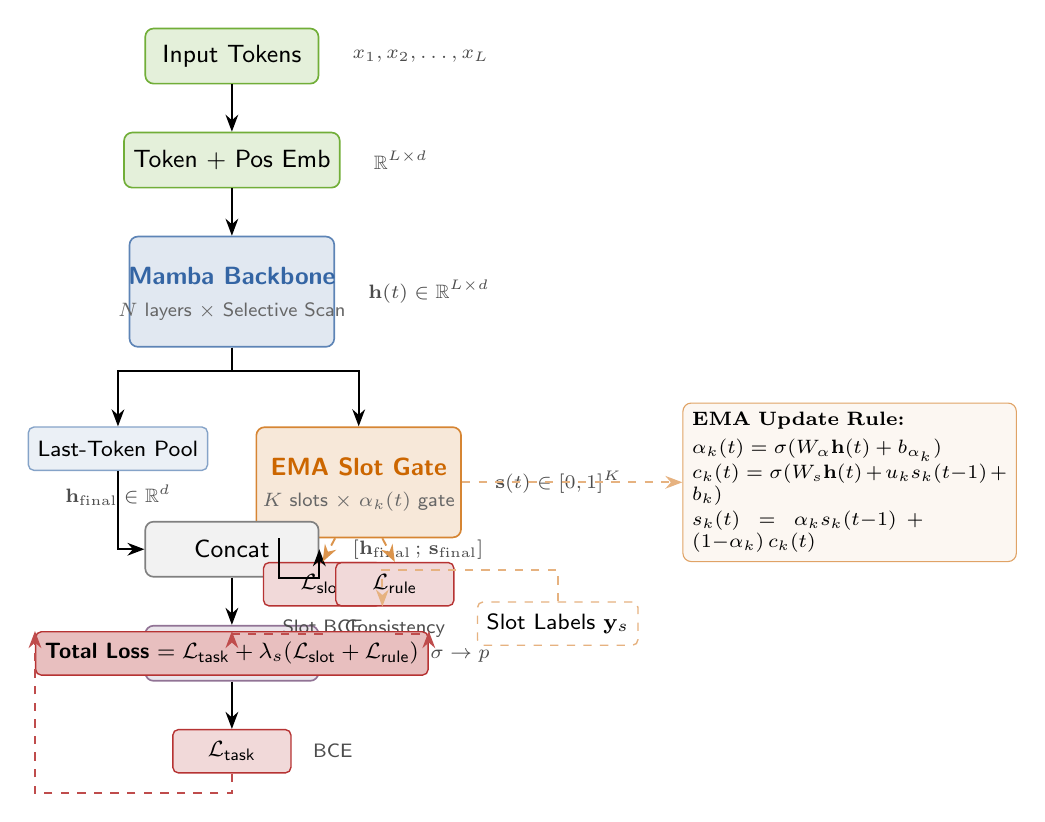
\begin{tikzpicture}[
    >=Stealth,
    block/.style={draw, rounded corners=3pt, minimum height=0.7cm,
                  minimum width=2.2cm, font=\small\sffamily,
                  line width=0.6pt},
    smallblock/.style={draw, rounded corners=2pt, minimum height=0.55cm,
                       minimum width=1.5cm, font=\footnotesize\sffamily,
                       line width=0.5pt},
    arr/.style={->, line width=0.7pt},
    darr/.style={->, line width=0.7pt, dashed},
    brace/.style={decorate, decoration={brace, amplitude=5pt, mirror}},
    lbl/.style={font=\scriptsize\sffamily, text=black!70},
]

% ══════════════════════════════════════
%  LEFT COLUMN: Main Forward Path
% ══════════════════════════════════════

% Input
\node[block, fill=embed!15, draw=embed!80] (input) {Input Tokens};
\node[lbl, right=0.3cm of input] {$x_1, x_2, \ldots, x_L$};

% Token + Position Embedding
\node[block, fill=embed!15, draw=embed!80, below=0.6cm of input] (emb)
    {Token + Pos Emb};
\node[lbl, right=0.3cm of emb] {$\mathbb{R}^{L \times d}$};

% Mamba Backbone (stacked)
\node[block, fill=mamba!15, draw=mamba!80, below=0.6cm of emb,
      minimum width=2.6cm, minimum height=1.4cm] (mamba) {};
\node[font=\small\sffamily\bfseries, text=mamba] at ([yshift=0.2cm]mamba.center)
    {Mamba Backbone};
\node[font=\scriptsize\sffamily, text=black!60] at ([yshift=-0.25cm]mamba.center)
    {$N$ layers $\times$ Selective Scan};
\node[lbl, right=0.3cm of mamba] {$\mathbf{h}(t) \in \mathbb{R}^{L \times d}$};

% Split point
\coordinate (split) at ([below=0.6cm]mamba.south);

% Last-token pooling
\node[smallblock, fill=mamba!10, draw=mamba!60,
      below left=1.0cm and 0.3cm of mamba.south] (pool)
    {Last-Token Pool};
\node[lbl, below=0.05cm of pool] {$\mathbf{h}_{\mathrm{final}} \in \mathbb{R}^d$};

% Slot Gate
\node[block, fill=slot!15, draw=slot!80, minimum width=2.6cm,
      minimum height=1.4cm, below right=1.0cm and 0.3cm of mamba.south] (slotgate) {};
\node[font=\small\sffamily\bfseries, text=slot] at ([yshift=0.2cm]slotgate.center)
    {EMA Slot Gate};
\node[font=\scriptsize\sffamily, text=black!60] at ([yshift=-0.25cm]slotgate.center)
    {$K$ slots $\times$ $\alpha_k(t)$ gate};
\node[lbl, right=0.3cm of slotgate] {$\mathbf{s}(t) \in [0,1]^K$};

% Concatenation
\node[block, fill=black!5, draw=black!50, below=2.2cm of split] (concat)
    {Concat};
\node[lbl, right=0.3cm of concat]
    {$[\mathbf{h}_{\mathrm{final}}\,;\,\mathbf{s}_{\mathrm{final}}]$};

% Answer Head
\node[block, fill=head!15, draw=head!80, below=0.6cm of concat] (head)
    {Answer Head};
\node[lbl, right=0.3cm of head] {MLP $\to \sigma \to p$};

% Task Loss
\node[smallblock, fill=loss!15, draw=loss!80, below=0.6cm of head] (ltask)
    {$\mathcal{L}_{\text{task}}$};
\node[lbl, right=0.15cm of ltask] {BCE};

% ══════════════════════════════════════
%  RIGHT COLUMN: Slot Details + Losses
% ══════════════════════════════════════

% EMA Equation box
\node[draw=slot!60, rounded corners=3pt, fill=slot!5,
      font=\scriptsize, text width=4.0cm, align=left,
      right=2.8cm of slotgate]
    (ema_eq) {%
    \textbf{EMA Update Rule:}\\[2pt]
    $\alpha_k(t) = \sigma(W_\alpha \mathbf{h}(t) + b_{\alpha_k})$\\[1pt]
    $c_k(t) = \sigma(W_s \mathbf{h}(t) + u_k s_k(t{-}1) + b_k)$\\[1pt]
    $s_k(t) = \alpha_k s_k(t{-}1) + (1{-}\alpha_k)\,c_k(t)$
    };

% Logic Losses
\node[smallblock, fill=loss!15, draw=loss!80,
      below left=0.3cm and -0.3cm of slotgate.south] (lslot)
    {$\mathcal{L}_{\text{slot}}$};

\node[smallblock, fill=loss!15, draw=loss!80,
      below right=0.3cm and -0.3cm of slotgate.south] (lrule)
    {$\mathcal{L}_{\text{rule}}$};

\node[lbl, below=0.05cm of lslot] {Slot BCE};
\node[lbl, below=0.05cm of lrule] {Consistency};

% Slot labels input (dashed)
\node[smallblock, fill=white, draw=slot!50, dashed,
      right=1.2cm of lslot, yshift=-0.5cm] (slabels)
    {Slot Labels $\mathbf{y}_s$};

% ══════════════════════════════════════
%  ARROWS
% ══════════════════════════════════════

% Forward path
\draw[arr] (input) -- (emb);
\draw[arr] (emb) -- (mamba);

% Split from Mamba
\draw[arr] (mamba.south) -- ++(0,-0.3cm) -| (pool.north);
\draw[arr] (mamba.south) -- ++(0,-0.3cm) -| (slotgate.north);

% Pool and slot to concat
\draw[arr] (pool.south) |- (concat.west);
\draw[arr] (slotgate.south west) ++(0.3cm,0) -- ++(0,-0.5cm) -| (concat.east);

% Concat to head
\draw[arr] (concat) -- (head);
\draw[arr] (head) -- (ltask);

% Slot gate to losses
\draw[darr, slot!70] (slotgate.south) +(-0.3cm,0) -- (lslot.north);
\draw[darr, slot!70] (slotgate.south) +(0.3cm,0) -- (lrule.north);

% EMA equation arrow
\draw[darr, slot!50] (slotgate.east) -- (ema_eq.west);

% Slot labels arrow
\draw[darr, slot!50] (slabels.north) -- ++(0,0.4cm) -| (lslot.south east);

% Total Loss brace
\node[smallblock, fill=loss!25, draw=loss!80, 
      below=3.6cm of split, minimum width=3.5cm] (ltotal)
    {\textbf{Total Loss} $= \mathcal{L}_{\text{task}} 
     + \lambda_s (\mathcal{L}_{\text{slot}} + \mathcal{L}_{\text{rule}})$};

\draw[darr, loss!70] (ltask.south) -- ++(0,-0.25cm) -| (ltotal.north west);
\draw[darr, loss!70] (lslot.south) ++(0,-0.35cm) -| (ltotal.north);
\draw[darr, loss!70] (lrule.south) ++(0,-0.35cm) -| (ltotal.north east);

\end{tikzpicture}
\end{document}
